%
% einleitung.tex -- Einleitung und Motivation
%
% (c) 2026 Baris Catan, OST Ostschweizer Fachhochschule
%
% !TEX root = ../../buch.tex
% !TEX encoding = UTF-8
%
\section{Eine harmlose Frage
\label{elliptisch:section:einleitung}}
\kopfrechts{Eine harmlose Frage}

Wir beginnen dieses Kapitel mit einer Frage, die einfacher klingt,
als sie ist.
Wie lang ist der Umfang einer Ellipse?
Für den Kreis mit Radius $r$ genügt die Parametrisierung
$(x,y) = (r\cos t,\, r\sin t)$.
Wegen $\sin^2 t + \cos^2 t = 1$ fällt die Wurzel im Bogenelement weg
und es bleibt
\begin{equation}
U
=
\int_0^{2\pi} \sqrt{\dot x^2 + \dot y^2}\,dt
=
\int_0^{2\pi} \sqrt{r^2\sin^2 t + r^2\cos^2 t}\,dt
=
\int_0^{2\pi} r\,dt
=
2\pi r.
\label{elliptisch:equation:kreisumfang}
\end{equation}

Dieselbe Rechnung führen wir nun für die Ellipse mit den Halbachsen
$a \ge b$ durch, parametrisiert durch
$(x,y) = (a\cos t,\, b\sin t)$
(siehe Abbildung~\ref{fig:elliptisch:ellipse}).
\begin{figure}
	\centering
	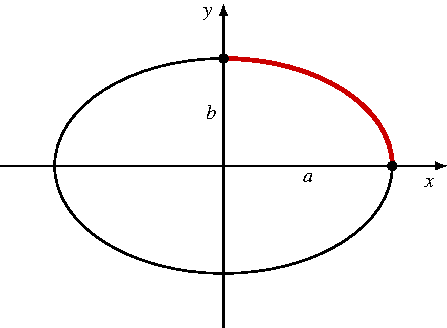
\includegraphics[width=0.6\textwidth]{papers/elliptisch/images/ellipse.pdf}
	\caption{Die Ellipse mit den Halbachsen $a$ und $b$.
	Hervorgehoben ist der Bogen im ersten Quadranten, der volle
	Umfang ist aus Symmetriegründen das Vierfache.}
	\label{fig:elliptisch:ellipse}
\end{figure}

Das Bogenelement ist
\begin{equation}
ds
=
\sqrt{\dot x^2 + \dot y^2}\,dt
=
\sqrt{a^2\sin^2 t + b^2\cos^2 t}\,dt
=
a\,\sqrt{1 - k^2\cos^2 t}\,dt,
\qquad
k^2 = \frac{a^2-b^2}{a^2},
\label{elliptisch:equation:bogenelement}
\end{equation}
wobei $k$ die numerische Exzentrizität ist
\cite{elliptisch:mueller-spezielle}, später auch Modul
genannt.
\index{Ellipse}%
\index{Exzentrizitat@Exzentrizität}%
Bemerkenswert ist, dass diesmal die Wurzel nicht verschwindet.
Wegen der Symmetrie der Ellipse genügt der erste Quadrant, der
volle Umfang
\begin{equation}
U
=
4a \int_0^{\pi/2} \sqrt{1 - k^2\cos^2 t}\,dt
\label{elliptisch:equation:umfangcos}
\end{equation}
ist das Vierfache davon.
Die Substitution $t \mapsto \frac{\pi}{2} - t$ bildet das Intervall
$[0, \pi/2]$ auf sich ab und vertauscht $\cos^2$ mit $\sin^2$.
Somit erhalten wir
\begin{equation}
U
=
4a \int_0^{\pi/2} \sqrt{1 - k^2\sin^2 t}\,dt.
\label{elliptisch:equation:umfang}
\end{equation}
Für den Kreis ist $a = b = r$, also $k = 0$, eingesetzt in
\eqref{elliptisch:equation:umfang} liefert
$U = 4a \cdot \frac{\pi}{2} = 2\pi r$, wie erwartet.
Wie sich herausstellen wird, hat das Integral
\eqref{elliptisch:equation:umfang} jedoch keine elementare Stammfunktion.

\subsection{Existenz und Darstellbarkeit}
\begin{satz}[Hauptsatz der Differential- und Integralrechnung]
Ist $f$ stetig, dann ist $F(x) = \int_a^x f(t)\,dt$
differenzierbar mit $F' = f$, insbesondere besitzt $f$ eine
Stammfunktion.
\end{satz}
Über die Existenz einer Stammfunktion muss man also nie streiten.
Ganz anders sieht es mit der \emph{Darstellbarkeit} aus.
Ob sich $F$ als endliche Formel aus Polynomen, Wurzeln, $\exp$,
$\log$ und den trigonometrischen Funktionen schreiben lässt,
ist eine völlig andere Frage.
Existenz heisst nicht Darstellbarkeit.
Funktionen, die aus Polynomen, Wurzeln, $\exp$, $\log$ und den
trigonometrischen Funktionen zusammengesetzt sind, heissen
\emph{elementar}, der Begriff wird weiter unten präzisiert und ist
ausführlich in Abschnitt~\ref{buch:intalg:section:elementar}
behandelt.
Drei Beispiele zeigen, wie weit Existenz und Darstellbarkeit
auseinanderliegen können.

Integranden mit der Wurzel aus einem quadratischen Polynom sind
stets elementar integrierbar, zum Beispiel
\begin{equation}
\int \sqrt{x^2+1}\,dx
=
\frac{1}{2}\left(x\sqrt{x^2+1} + \operatorname{arsinh} x\right),
\label{elliptisch:equation:wurzelstandard}
\end{equation}
dessen Stammfunktion handhabbar ist, um damit weiterzurechnen.
Abschnitt~\ref{buch:intalg:section:wurzel} zeigt, dass dies für
jedes quadratische Polynom unter der Wurzel gelingt.

Schon der Integrand $\sqrt{\tan x}$ zeigt jedoch, dass aus
elementar lösbar nicht brauchbar folgt.
Die Substitution $u = \sqrt{\tan x}$ macht den Integranden
rational,
\begin{equation}
\int \sqrt{\tan x}\,dx
=
\int \frac{2u^2}{1+u^4}\,du,
\label{elliptisch:equation:tanxrational}
\end{equation}
und die Partialbruchzerlegung über die Faktorisierung
$1+u^4 = (u^2-\sqrt{2}u+1)(u^2+\sqrt{2}u+1)$
garantiert eine elementare Stammfunktion.
Ein Computeralgebrasystem liefert sie auch, nämlich
\begin{equation}
\frac{\sqrt{2}}{4}
\log\frac{\tan x-\sqrt{2}\sqrt{\tan x}+1}
        {\tan x+\sqrt{2}\sqrt{\tan x}+1}
+
\frac{\sqrt{2}}{2}\arctan\left(\sqrt{2}\sqrt{\tan x}-1\right)
+
\frac{\sqrt{2}}{2}\arctan\left(\sqrt{2}\sqrt{\tan x}+1\right).
\label{elliptisch:equation:tanxmonster}
\end{equation}
Der Ausdruck ist so unhandlich, dass er für praktische Zwecke
kaum etwas nützt.

Beim dritten Beispiel versagt die elementare Integration
vollständig.
Für
\begin{equation}
\int e^{-x^2}\,dx
\label{elliptisch:equation:expx2}
\end{equation}
lässt sich beweisen, dass keine elementare Stammfunktion existiert,
der Beweis wird in Abschnitt~\ref{buch:intalg:section:risch}
geführt.
An dieser Stelle ist die Konsequenz wichtiger als der Beweis.
Wenn keine elementare Stammfunktion existiert, bleibt nur, dem
Integral einen Namen zu geben und es selbst zur Funktion zu
erklären.
Für dieses Integral ist das geschehen, die Fehlerfunktion
\begin{equation}
\operatorname{erf}(x)
=
\frac{2}{\sqrt{\pi}} \int_0^x e^{-t^2}\,dt
\label{elliptisch:equation:erfx}
\end{equation}
ist nichts anderes als die Stammfunktion von $e^{-x^2}$ in
normierter Form.
\index{Fehlerfunktion}%
Dasselbe Prinzip steckt hinter der Definition
$\log x = \int_1^x \frac{dt}{t}$,
und genau derselbe Schritt wird in diesem Kapitel mit den
elliptischen Integralen vollzogen.
Was nicht elementar integrierbar ist, wird zur neuen Funktion.
Die Frage, welche Integranden eine elementare Stammfunktion
besitzen, ist damit keine Frage der Analysis, sondern der Algebra.

\subsection{Elementare Funktionen}
Der Begriff der elementaren Funktion, den wir bisher nur
umgangssprachlich verwendet haben, lässt sich algebraisch fassen.
Ausgangspunkt ist der Körper $F_0 = \mathbb{Q}(x)$ der rationalen
Funktionen zusammen mit der gewöhnlichen Ableitung.
In jedem weiteren Schritt kommt eine einzelne neue Funktion
$\vartheta$ dazu, die über dem bisherigen Körper algebraisch ist oder
zu einem $v$ des bisherigen Körpers die Gleichung $\vartheta' = v'/v$
erfüllt, also ein Logarithmus ist, oder die Gleichung
$\vartheta'/\vartheta = v'$, also eine Exponentialfunktion
(siehe Abschnitt~\ref{buch:intalg:section:elementar}).
So entsteht ein \emph{Turm}
\begin{equation}
F_0 \subset F_1 \subset \dots \subset F_N,
\qquad
F_i = F_{i-1}(\vartheta_i),
\label{elliptisch:equation:koerperturm}
\end{equation}
von Körpererweiterungen.
Jeder Körper $F_i$ darin ist eine Erweiterung seines Vorgängers um
genau eine neue Funktion $\vartheta_i$.
Eine Funktion heisst \emph{elementar}, wenn sie sich in endlich
vielen solchen Schritten aufbauen lässt
(Abbildung~\ref{fig:elliptisch:koerperturm}).
\index{elementare Funktion}%
\index{Korperturm@Körperturm}%
\begin{figure}
	\centering
	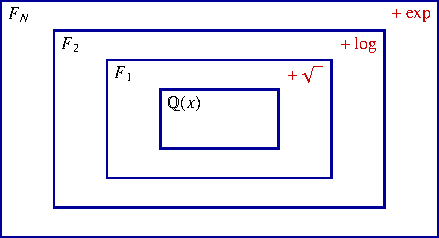
\includegraphics[width=0.7\textwidth]{papers/elliptisch/images/koerperturm.pdf}
	\caption{Eine elementare Funktion liegt in einem endlichen Turm
	von Körpererweiterungen, ausgehend von den rationalen Funktionen
	$\mathbb{Q}(x)$.
	In jedem Schritt kommt eine Wurzel, ein Logarithmus oder eine
	Exponentialfunktion dazu.}
	\label{fig:elliptisch:koerperturm}
\end{figure}

Die Sinus- und Kosinusfunktion fehlen in dieser Aufzählung nicht,
sie stecken über $\sin x = (e^{ix}-e^{-ix})/2i$ bereits in den
exponentiellen Schritten.
Die Wurzel $\sqrt{p(x)}$ ist ein algebraischer Schritt, denn sie
erfüllt die Gleichung $\vartheta^2 - p(x) = 0$ über
$\mathbb{Q}(x)$.
Alles, was sich als endliche Formel hinschreiben lässt, ist damit
erfasst.

\subsection{Der Satz von Liouville}
Ableiten führt aus einem solchen Turm nie heraus.
Liegt $f$ in einem der Körper $F_i$, dann liegt auch $f'$ wieder in
$F_i$, denn Summen-, Produkt- und Kettenregel erzeugen nur
Ausdrücke in bereits vorhandenen Elementen.
Beim Integrieren gilt das nicht, schon $\int dx/x = \log x$ verlässt
den Körper $\mathbb{Q}(x)$.
Die Frage ist also, wie weit man im Turm hinaufsteigen muss, um eine
Stammfunktion zu erreichen.
Liouville hat sie ab 1833 beantwortet
\cite{elliptisch:wiki-liouville}, und die
Antwort fällt enger aus, als man erwarten würde.
\index{Liouville, Satz von}%
\begin{satz}[Prinzip von Liouville]
\label{elliptisch:satz:liouville}
Sei $F$ ein Funktionenkörper mit Konstantenkörper $C$ und $f \in F$.
Besitzt $f$ eine Stammfunktion in einer elementaren Erweiterung von
$F$ mit demselben Konstantenkörper, dann gibt es Elemente
$v_0, v_1, \dots, v_n \in F$ und Konstanten
$c_1, \dots, c_n \in C$ mit
\begin{equation}
\int f\,dx
=
v_0 + \sum_{i=1}^n c_i \log v_i.
\label{elliptisch:equation:liouville}
\end{equation}
\end{satz}
Der Beweis wird in Abschnitt~\ref{buch:intalg:section:liouville}
geführt.
An dieser Stelle interessiert uns, was die Aussage leistet.

Ohne diesen Satz müsste die Stammfunktion in einer beliebig grossen
elementaren Erweiterung von $F$ gesucht werden, mit beliebig vielen
neuen Wurzeln, Exponentialfunktionen und ineinander geschachtelten
Logarithmen.
Somit ist die Art, wie die Stammfunktion aussieht, relativ starr.
Die Bausteine $v_0$ und $v_i$ liegen bereits in $F$, hinzu kommen
einzig die Logarithmen $\log v_i$, und deren Vorfaktoren $c_i$ sind
Konstanten.
Eine Exponentialfunktion, die im Integranden nicht vorkommt, kann in
der Stammfunktion also gar nicht auftauchen, und ein Logarithmus
eines Logarithmus ebenso wenig.
Der Turm über $F$, in dem die Stammfunktion zu suchen ist, hat damit
nur noch eine einzige Etage.

Zum Rechnen eignet sich die abgeleitete Fassung
\begin{equation}
f
=
v_0' + \sum_{i=1}^n c_i \frac{v_i'}{v_i}
\label{elliptisch:equation:liouvilleableitung}
\end{equation}
besser, denn sie enthält kein Integral mehr und ist eine Gleichung
innerhalb von $F$.
Aus der Existenzfrage wird damit eine Rechnung.
Man setzt die Form \eqref{elliptisch:equation:liouvilleableitung} mit
unbekannten $v_i$ und $c_i$ an und vergleicht Koeffizienten.
Geht die Rechnung auf, ist die Stammfunktion gefunden.
Führt sie auf einen Widerspruch, so ist bewiesen, dass keine
elementare Stammfunktion existiert.
Auf diesem Weg wird in
Abschnitt~\ref{buch:intalg:section:risch} gezeigt, dass $e^{-x^2}$
keine elementare Stammfunktion besitzt.
Risch hat das Verfahren in den Sechzigerjahren zu einem Algorithmus
ausgebaut \cite{elliptisch:risch}, der die Frage in endlich vielen
Schritten entscheidet.
Abschnitt~\ref{buch:intalg:section:risch} stellt ihn ausführlich dar.
Dieser Risch-Algorithmus steckt heute im Kern der
Integrationsroutinen von Computeralgebrasystemen.
\index{Risch-Algorithmus}%
